\section{Programmtests}
\FloatBarrier

\paragraph{Erkl"arung des Toolkits}
Um effektiv Tests zum Einlesen sowie Ausgeben von Spielst"anden aus einer .txt Datei gestalten zu k"onnen, wurde eine Klasse geschrieben, welche dies erleichtern soll. Sie nennt sich \emph{TestToolkit}. Bei der Erstellung habe ich mich stark an dem Toolkit aus der "Ubung \emph{Algorithmen und Datenstrukturen} orientiert. Das gegebene Toolkit ist allerdings nur in der Lage unter einer Unix-Umgebung Dateivergleiche durchzuf"uhren, da das Programm allerdings unter Windows entwickelt wurde, mussten viele Methoden ausgetauscht werden. Die Datei aus Algorithmen und Datenstrukturen befindet sich ebenfalls im Verzeichnis des Anhangs, kann aber auch wieder alternativ "uber die Lesezeichen- bzw. die Anlage"ubersicht betrachtet werden. 

\embedfilesetup{mimetype=application/octet-stream}
\embedfile{programmierhandbuch/programmtests/TestToolkit.java}

Neben einer Festlegung welcher Dateityp bearbeitet werden kann, liefert diese Klasse vor allem einen Pfad an dem s"amtliche Testdateien zu finden sind. Dies geschieht ("ahnlich wie beim Logger) mit einem Formatstring. Um Testdateien zuallererst in Form eines Strings zu lesen wird die Methode \emph{readAsString} verwendet \lstref{lst:testToolkit_readAsString}. Diese verwendet allerdings nur die bereits implementierte Methode der Loader-Klasse. Es war mir trotzdem wichtig sie hier mit aufzunehmen, um eine gemeinsame Schnittstelle f"ur alle Tests der Dateiverarbeitung zu schaffen. In der Methode \emph{read} wird diese Methode aufgerufen um einen Game Konstruktor zu f"ullen und ein vollwertiges Spiel zur"uckzugeben. 

Eine weitere Funktionalit"at des Toolkits besteht darin zwei gegebene Dateien mit dem selben Namen auf ihre Gleichheit zu pr"ufen \lstref{lst:testToolkit_assertFilesEqual}. Dies geschieht, indem beide Dateien aus den gegebenen Verzeichnissen (\emph{results} sowie \emph{expected\_results}) als Strings ausgelesen und anschlie"send per assertEquals verglichen werden. Die Methode \emph{writeAndAssert} verh"alt sich hier sehr "ahnlich, hierbei wird nur erst das gegebene Spiel in eine Datei geschrieben bevor die assertFilesEqual der Klasse aufgerufen wird. 
\begin{lstlisting}[float,style=CodeHighlighting,caption=TestToolkit - readAsString,label=lst:testToolkit_readAsString]
public static String readAsString(String filename) {
    try {
        File file = new File(String.format(PATH_FORMAT, filename));
        return Loader.getInstance().openGivenFile(file.getPath());
    } catch (FileNotFoundException e) {
        return e.getMessage();
    }
}
\end{lstlisting}
\begin{lstlisting}[float,style=CodeHighlighting,caption=TestToolkit - assertFilesEqual,label=lst:testToolkit_assertFilesEqual]
public static void assertFilesEqual(String filename) {
    try {
        File fileResult = new File("test" + File.separator + "fileTests" + File.separator
                + "results" + File.separator + filename + ".txt");
        File fileExpectedResult = new File("test" + File.separator + "fileTests" 
        		+ File.separator + "expected_results" + File.separator + filename 
        		+ ".txt");
        Assert.assertEquals(Loader.openGivenFile(fileExpectedResult), 
        		Loader.openGivenFile(fileResult));
    } catch (FileNotFoundException e) {
        assertTrue(false);
    }
}
\end{lstlisting}

\subparagraph{Beschreibung der Testf"alle}
Um Testf"alle gestalten zu k"onnen ohne jedes Mal eine Grafische Benutzeroberfl"ache starten zu m"ussen habe ich "ahnlich wie in der Bonusaufgabe eine Klasse namens \emph{FakeGUI} erstellt, welche genau wie die JavaFXGUI das Interface \emph{GUIConnector} implementiert.

Um sinnvoll das Ein- sowie Auslesen von Dateien testen zu k"onnen wurde folgende Ordnerstruktur gew"ahlt: Im Ordner namens \glqq test\grqq befindet sich ein Unterordner namens \glqq fileTests\grqq {}. Dies ist der Oberordner, in welchem sich alle Testdateien zum Dateieinlesen sowie ausgeben befinden. Die Dateien mit dem Pr"afix \glqq inv\_\grqq {} spiegeln invalide, w"ahrend die mit dem Pr"afix \glqq val\_\grqq {} valide Dateien wiederspiegeln. Da im Converter drei unterschiedliche Komponenten generiert werden, wurden die Testf"alle hieran angelehnt. Es gibt also jeweils Testf"alle f"ur Fehler im Spielbrett, den B"anken und dem Stapel. Zu validen Spielsituationen gibt es deutlich weniger Tests, da viele der Situationen in den Unittests zu den einzelnen Datenstrukturen bereits behandelt wurden. Invalide Dateitests laufen immer nach dem selben Schema ab \lstref{lst:test_noTagOpenerAtBeginningOfDoc}. Es wird die erwartete Fehlermeldung in eine Variable gespeichert. Anschlie"send wird der String aus der Datei mittels \emph{readAsString} aus der Toolkit-Klasse gelesen und dem Converter "ubergeben um dieselbe Situation zu erzeugen wie es beim Einlesen im normalen Spielverlauf der Fall ist. Im letzten Schritt werden String-Ausagbe mit der Fehlermeldung vom Anfang verglichen. 

Etwas komplexer gestalten sich die Tests bez"uglich der validen Spielsituationen. Hierbei wird ein Spiel mit den erwarteten Daten erzeugt. Danach wird die Methode \emph{read} der TestToolkit-Klasse verwendet um ein Spiel zu erzeugen. Diese wurde bereits im vorherigen Absatz erw"ahnt, denn sie ruft lediglich die readAsString-Methode auf, um den generierten String dem Game-Konstruktor zu "ubergeben. Wie der Einleseprozess im Detail funktioniert wird in der Erkl"arung der Converter-Klasse beschrieben (siehe Abschnitt \ref{spar:converter_ablauf}, S. \pageref{spar:converter_ablauf}). Das so generierte Spiel wird mit einem Spiel verglichen, welches vorher \glqq per Hand\grqq {} erzeugt wurde. Hierzu wird die \emph{equals}-Methode der \emph{Game}-Klasse verwendet, welche "uber assertEquals angesteuert wird. Im Anschluss wird das gelesene Spiel einmal abgespeichert und per \emph{writeAndAssert} von der TestToolkit-Klasse "uberpr"uft ob die Datei den selben Spielstand enth"alt. In der \emph{writeAndAssert}-Methode wird zuerst eine neue Datei mit dem gegebenen Namen in dem Unterordner \glqq results\grqq  erstellt. Anschlie"send ist der Loader zum Abspeichern zust"andig. Wie der Loader vorgeht um eine Datei abzurufen wird im Abschnitt \ref{par:loader}, S. \pageref{par:loader} n"aher erl"autert. 
In Abbildung \ref{fig:testCoverage} - \nameref{fig:testCoverage} ist au"serdem eine Auflistung der Testcoverage zu sehen.

\subparagraph{Auflistung wichtiger Testf"alle}
In der folgenden detailierten Auflistung (ValidFileReadTests) werde ich mich auf die Tests, welche sich mit dem Dateieinlesen besch"afftigen, beschr"anken. S"amtliche andere Testklassen sind relativ grundlegend gestaltet, dass es kein Problem sein sollte nachzuvollziehen was genau gepr"uft wird. 

\bigbreak

\begin{tabular}{|p{2cm}|p{7cm}|p{2cm}|p{2cm}|}
	\hline
	Name & Testfall & erwartetes Ergebnis & erzieltes Ergebnis \\
	\hline
	\hline
	newGame noNextBankYet & Das Spiel wurde w"ahrend des initialen Selektierens abgespeichert. Es wurde lediglich die \emph{currentRoundBank} geladen. Hierbei hat noch kein Spieler eine Auswahl getroffen. Dies ist der Zustand welcher nach dem Aufruf der startGame-Methode vorzufinden ist. Es wird ein Spiel generiert und mit dieser Methode begonnen. Anschlie"send wird das Spiel mit selben Namen (wie der Test) aus dem Expected-Ordner geladen und mit dem Spiel verglichen. & Das eingelesene und generierte Spiel sind gleich. & Das eingelesene und generierte Spiel sind gleich. \\
		
	fullCurrBank fullStack & Spiel wurde w"ahrend einer standardm"a"sigen Runde abgespeichert. Es wird erwartet eine, von allen Spielern selektierte \emph{currentRoundBank}, und eine nicht selektierte \emph{nextRoundBank}, vorzufinden. Au"serdem wurden die Spielfelder der Spieler bereits ver"andert und m"ussen eingelesen werden. Im Testaufruf wird die \emph{equals}-Methoder der Game-Klasse aufgerufen, da diese alle beteiligten Teilkomponenten pr"uft. & Das eingelesene und generierte Spiel sind gleich. & Das eingelesene und generierte Spiel sind gleich. \\
	
	noStack & Es wird ein Spiel generiert, welches einen leeren Beutel besitzt. S"amtliche Felder der Spieler m"ussen geladen werden und es werden die letzten Z"uge der noch fehlenden Spieler absolviert. Wichtig hierbei, der menschliche Spieler muss seinen letzten Zug ausf"uhren, der Domino befindet sich allerdings noch auf der Bank. & Das eingelesene und generierte Spiel sind gleich. & Das eingelesene und generierte Spiel sind gleich. \\
	
	lastTurnIn- \newline RotBox & Es wird eine "ahnliche Situation wie im vorherigen Test generiert. Allerdings wurde hierbei der Domino der Bank bereits in die Rotationsbox des menschlichen Spielers geladen. Wie bei allen dieser Testf"alle wird auch hier wieder das Spiel mit der gleichnamigen Datei verglichen. & Das eingelesene und generierte Spiel sind gleich. & Das eingelesene und generierte Spiel sind gleich. \\	
	\hline
\end{tabular}

\begin{figure}
	\centering
	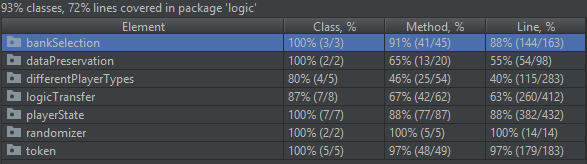
\includegraphics{pics/testCoverage}
	\caption{Testcoverage}
	\label{fig:testCoverage}
\end{figure}

\begin{lstlisting}[float,style=CodeHighlighting,caption=InvalidFileReadTests - test\_noTagOpenerAtBeginningOfDoc,label=lst:test_noTagOpenerAtBeginningOfDoc]
@Test
public void noTagOpenerAtBeginningOfDoc() {
    String expOutput = WrongTagException.DEFAULT_MESSAGE;
    String fileOutput = TestToolkit.readAsString("inv_noTagOpenerAtBeginningOfDoc");
    String actOutput = new Converter().readStr(new FakeGUI(), fileOutput);
    assertEquals(expOutput, actOutput);
}
\end{lstlisting}

\subparagraph{"Uberblick "uber weitere Testklassen}
Um noch einen "Uberblick "uber s"amtliche andere Testklassen zu geben folgt eine kurze Zusammenfassung der jeweiligen Klassen. 

\begin{longtable}{|p{1.5cm}|p{7.5cm}|p{2cm}|p{2cm}|}
	\hline
	Name & Testfall & erwartetes Ergebnis & erzieltes Ergebnis \\
	\hline

	
	BankTest & 
Konstruktor: Stringeingaben sowie Entry-Arrays werden als Eingabe getestet. 
	\newline Selektieren: Es werden Pl"atze auf der Bank selektiert. Anschlie"send werden die Spielerreferenzen verglichen.
	\newline Getter: B"anke werden erstellt und gew"unschte Objekte per Getter geholt und verglichen.
	\newline Zuf"alliges Ziehen aus dem Stapel: Eine Bank wird gef"ullt, allerdings wird der Bank ein PseudoRandom Objekt "ubergeben. Mit diesem ist es m"oglich stets dieselbe Auswahl zu treffen. 
	& Die generierten B"anke enthalten die erwarteten Eintr"age. 
 	& Die generierten B"anke enthalten die erwarteten Eintr"age. \\
 	
 	\hline 
 	
	EntryTest
	& Es wrid die String-Repr"asentation sowie die Equals Methode eine Eintrags getestet. Mit entsprechendem Konstruktor werden die Tests geladen und per toString / equals gepr"uft. 
	& Die Eintr"age entsprechen der erwarteten String-Repr"asen- \newline tation bzw. dem generierten Referenzobjekt.
	& Die Eintr"age entsprechen der erwarteten String-Repr"asen- \newline tation bzw. dem generierten Referenzobjekt. \\
	
 	\hline 
 	
 	Game- \newline Loading- \newline Construc- \newline torTest und GameTest
 	& Hierbei wird genauso vorgegagangen wie bei den \emph{ValidFileReadTests}, es wird allerdings nicht gegen eine Datei getestet, sondern s"amtilche Referenzobjekte werden vor Ort erstellt und auf Gleichheit mit dem erstellten Spiel getestet. 
 	& S"amtliche Teilkomponenten entsprechen den Komponenten im Spiel. 
 	& S"amtliche Teilkomponenten entsprechen den Komponenten im Spiel. \\
 	
  	\hline 
 	
	Board- \newline Test
	& Es werden per diverse Spielsituationen per String-Eingabe im Konstruktor erzeugt. Da dies in erster Linie als Datenobjekt fungiert werden "uber entsprechende Getter Werte verglichen. 
	& Die angeforderten Werte entsprechen den erwarteten. 
	& Die angeforderten Werte entsprechen den erwarteten. \\
	
 	\hline 
	
	Default- \newline AIPlayer- \newline Test
	& Es wird ein k"unstlicher Spieler erzeugt und mit entsprechenden Spielsituationen konfrontiert. Dabei selektiert er jedes Mal von der Bank, da er hiermit nicht nur einen Domino w"ahlt, sondern diesen auch gleichzeitig positioniert. Diverse Teilaspekte werden mit jedem Test behandelt obwohl die Tests alle relativ "ahnlich aussehen. Es sei noch erw"ahnt, dass bei einem Konstruktoraufruf mit einer String-Eingabe gleichzeitig die Distrikte aufgebaut werden. Daher ist es auch hier m"oglich die Distrikte zu pr"ufen. 
	& Auf Board des Spielers wird der erwartete Domino gesetzt. 
	& Auf Board des Spielers wird der erwartete Domino gesetzt. \\
	
	\hline 
 	
 	District- \newline Test
	& Hierbei wird ein einzelner Distrikt getestet, wichtig hierbei sind insbesondere das Hinzuf"ugen neuer Distriktelemente sowie das Zusammenf"uhren mehrerer Distrikte. Es werden Listen mit entsprechenden Referenzobjekten gebildet und verglichen. 
	& Die Liste der Referenzobjekte stimmt mit den generierten Werten "uberein. 
	& Die Liste der Referenzobjekte stimmt mit den generierten Werten "uberein. \\
	
	\hline 
 	
	Player- \newline Test
	& In dieser Klasse werden Spielerunspezifische Methoden getestet, ein Beispiel w"are das Verwerfen eines Dominos. Agiert ansonsten sehr "ahnlich zum DefaultAIPlayerTest. 
	& Auf Board des Spielers wird der erwartete Domino gesetzt. 
	& Auf Board des Spielers wird der erwartete Domino gesetzt. \\
	
	\hline 
	
	Domino- \newline Test
	& Diese Testklasse wurde bereits in der Bonusaufgabe gegeben und wurde meinerseits mit leichten Modifikationen "ubernommen. 
	& Die generierten Dominos entsprechen den Erwarteten. 
	& Die generierten Dominos entsprechen den Erwarteten. \\
 	
	\hline
	
\end{longtable}

